\documentclass[referee,sn-basic]{sn-jnl}% referee option is meant for double line spacing
%\documentclass[sn-mathphys]{sn-jnl}% Math and Physical Sciences Reference Style
\jyear{2022}%
\theoremstyle{thmstyleone}%
\newtheorem{theorem}{Theorem}%  meant for continuous numbers
\newtheorem{proposition}[theorem]{Proposition}%
\theoremstyle{thmstyletwo}%
\newtheorem{example}{Example}%
\newtheorem{remark}{Remark}%
\theoremstyle{thmstylethree}%
\newtheorem{definition}{Definition}%
\raggedbottom
\usepackage{makecell}
\usepackage{natbib}
\setcitestyle{aysep={}}

\begin{document}
\title[Y-chromosome degeneration due to speciation and founder effect]{Y-chromosome degeneration due to speciation and founder effect}
\author[1]{\fnm{Nian-Qin} \sur{Zhang}}

\author*[2]{\fnm{Yong-Jun} \sur{Zhang}}\email{yong.j.zhang@gmail.com}

\affil[1]{ \orgname{Southern Medical University}, \orgaddress{ \city{Guangzhou},  \country{China}}}

\affil*[2]{\orgdiv{Science college}, \orgname{Liaoning Technical University}, \orgaddress{\city{Fuxin}, \country{China}}}

\abstract{
The Y chromosome is often shorter than the X chromosome in the XY sex-determination system due to degeneration following Y recombination arrest. The classical paradigm suggests that degeneration is a process happening over time. However, there is a species-specific tendency that the more advanced a species is, the shorter the Y chromosome is. We suggest a degeneration mechanism that is associated with speciation. For species with large population sizes, equilibrium can be reached for mutant alleles due to mutation-selection balance. But when a new species arises, the Y chromosome may lose active genes when the founder effect plays a role. For example, suppose all the male founders of a species carry only a mutant allele of a particular gene on their Y chromosomes, then all the male offspring will only carry the same mutant allele instead of the wild-type allele, resulting in the loss of the active gene from the Y chromosome.
}
\keywords{sex\ chromosome, equilibrium, evolution, founder\ effect, bottleneck\ effect}

\maketitle

\section{Introduction}
Sex is one of the greatest inventions of life. It gives rise to offspring diversity; more importantly, it gives rise to chromosome recombination, allowing beneficial genes to accumulate. The suppression of recombination can trigger the degrading of sex chromosomes \citep{bachtrog2014sex,furman2020sex}.
Sex-determining mechanisms can be implemented in various ways. One way is XY sex-determination system, in which females have two X chromosomes and males have one X chromosome and one Y chromosome. The two sex chromosomes evolved from a pair of autosomes when one autosome acquired a male-determining gene (SRY) to become the Y chromosome, leaving the other autosome to become the X chromosome. The heterogeneity of the sex chromosome somehow suppresses the recombination of the sex chromosomes. As a result, the Y chromosome degrades. For example, the human Y chromosome has only three percent of its ancestral genes left \citep{skaletsky2003male}. A similar phenomenon is observed in another sex-determination system, the ZW system, in which the ZW genotype gives rise to females and the ZZ genotype gives rise to males, and the W chromosome tends to be shorter than the Z chromosome \citep{Zhou2014qi}.


It is still under study how recombination suppression causes Y-chromosome degeneration. One possible mechanism is Muller’s ratchet \citep{Muller1964, Ohno1967,charlesworth1978model}, according to which, every time a deleterious gene rises, it is an irreversible event because it cannot be repaired due to the lack of the recombination \citep{bachtrog2013chromosome}. Every time the Y chromosome accumulates a deleterious gene, it is an analogy that Muller's ratchet clicks, moving unidirectionally. However, Muller's ratchet may not click as frequently as expected for a large population.  

Other mechanisms may also play a role in Y degeneration \citep{bachtrog2008temporal}. The background selection model proposes that the Y chromosome loses variation due to neutral mutations being eliminated along with the deleterious mutation linked next to it \citep{charlesworth1993effect}. The genetic hitchhiking model proposes that the Y chromosome gradually loses its genetic activity because the frequency of deleterious mutations increases when it happens to be close to a beneficial mutation \citep{rice1987genetic}, e.g., SRY. Epigenetics effect may also play a role that the instability and divergence of {\it cis}-regulatory sequences in the non-recombining region may accelerate Y degeneration \citep{lenormand2020sex}. 


All these models share a common feature: the degeneration occurs over time or generations \citep{Charlesworth2021}. This assumption sparks fears that the human Y chromosome will become shorter and shorter and eventually vanish \citep{graves2006sex}. However, this assumption cannot accommodate the pattern that degeneration is rarely observed in cold-blooded vertebrates, in sharp contrast with birds and mammals. For example, a group of European tree frogs shows no divergence between the X and Y chromosomes even after they have evolved for millions of years \citep{stock2011ever}. Primitive species tend to have less degenerated sex chromosomes than advanced species \citep{gschwend2012sex}. In addition, the human Y chromosome has not lost any gene since the human and chimpanzee lineages diverged about 6 million years ago \citep{hughes2012strict}. 

The discrepancy between observations and theories demands an explanation \citep{Kratochvil2021}. One way to do so is to assume that the degeneration has been reversed from time to time, as suggested by some theories such as sex chromosome turnover \citep{schartl2004sex,miura2017sex} and occasional X-Y recombination \citep{perrin2009sex,stock2013low,rodrigues2018sex}. 

But the discrepancy also suggests that we may need a different model and assume the existence of equilibrium. One way to study equilibrium is the Hardy-Weinberg law \citep{johnston2019population}, which is a model able to calculate genotype frequencies from allele frequencies as long as the population is large, mating is at random, and mutation, selection, and migration are negligible. This law, in principle, does not consider mutation and natural selection; but reasonable results can still be obtained when extended to include them. Consider a locus with two alleles, G and g, and their equilibrium frequencies $p$ and $q$, respectively. For the scenario of autosomal locus, the population frequencies of genotypes GG, Gg, and gg are $p^2$, $2pq$, and $q^2$, respectively. When their relative fitnesses are 1, 1, and 0, respectively, there will be $q=\sqrt{\mu }$ due to mutation-selection balance, where $\mu$ is the mutation rate from G to g per generation. For the scenario of X-linked locus, the male genotypes are G and g, and when their corresponding fitnesses are 1 and 0, respectively, there will be $q\approx 3\mu$. 
Another way to study equilibrium is via an approach Haldane \citep{Haldane2004a} proposed in 1935. The approach does not assume the Hardy-Weinberg population. Instead, it lets genotype frequencies be determined directly by mutation-selection balance.

We follow Haldane's approach. We first study X-linked and autosomal alleles, which enable us to further study sex-linked alleles. After that, we do simulations for a small-sized population and explore the possibility of Y-chromosome degeneration via peripatric speciation and founder event.

\section{X-linked locus}
Consider an X-linked locus with alleles G and g. Let $\mu$ represent the mutation rate from G to g per generation, with no difference between males and females and no back mutation. Suppose the population is large and mating is at random. 
For females, the genotypes are GG, Gg, and gg. Let their relative fitnesses be 1, 1, and 0, respectively.
For males, the genotypes are G and g. Let their fitnesses be 1 and 0, respectively. In other words, the allele G is the functional wild-type allele, which is not dosage-sensitive, and the non-functional mutant allele g is recessive lethal. Let us denote the frequency of genotype Gg by $a$. The reproduction process is shown in Table \ref{X-linked}, where no mutation is considered.

\begin{table}[htp]
        \caption{Reproduction with no mutation considered. For males, the relative fitnesses of genotypes G and g are 1 and 0, respectively. For females, the relative fitnesses of genotypes GG, Gg, and gg are 1, 1, and 0, respectively. The frequencies of genotypes GG and Gg for parental generation are $1-a$ and $a$, respectively. \label{X-linked}
        }
        \begin{center}
                \begin{tabular}{ c!{\vrule width 1pt}c|c|c }
                        \hline
                        \vspace{-2mm}
                             &     &     &     \\
                      %\diaghead{2,2}{female}{male} & GG    & Gg    & gg    \\
                       & GG    & Gg    & gg    \\
                        & $1\!-\!a$ & $a$     &       \\
                        \vspace{-3mm} &       &     \\
			\noalign{\hrule height 1pt}
                        \vspace{-2mm}
                        &     &     &       \\
                        G      & \{ 2GG \} & \{ GG, Gg \}   &-      \\
                        1     & $1\!-\!a$  & $a$          &       \\
                        \vspace{-3mm}      &     &     &     \\
                        \hline
                        \vspace{-2mm}
                        &     &     &          \\
                        g     & -  & -          &       \\
                        \ \ \ \ \ 0\ \ \ \ \       &\ \ \ \ \ \ \ \ \ \ \ \ \  \ \ \ \ \ \ \ \ \ \ \ \ \    & \ \ \ \ \ \ \ \ \ \ \ \ \  \ \ \ \ \ \ \ \ \ \ \ \ \     & \ \    \ \ \         \\
                        \hline
                \end{tabular}
        \end{center}
\end{table}

When the mutation is taken into account, we need to make the following substitutions
\begin{equation}\label{GG}
  \begin{array}{lllll}
  {\rm GG}& \to 
  \begin{cases}
    {\rm GG}, &(1-\mu)^2,\\ {\rm Gg}, &2\mu(1-\mu),\\{\rm gg}, &\mu^2, 
  \end{cases}
  \end{array}
\end{equation}
\begin{equation}\label{Gg}
  \begin{array}{lllll}
  {\rm Gg}& \to 
  \begin{cases}
   {\rm Gg}, &(1-\mu),\\ {\rm gg}, &\mu.
  \end{cases}
  \end{array}
\end{equation}
Plugging Eqs. (\ref{GG}) and (\ref{Gg}) into Table (\ref{X-linked}),
we get
\begin{equation}
 \begin{array}{lll}
\vspace{2mm} N_{\rm GG}\propto&\left[2(1-a)+a\right](1-\mu)^2,\\
\vspace{2mm} N_{\rm Gg}\propto&\left[2(1-a)+a\right]2\mu(1-\mu)+ a(1-\mu),
  \end{array}
  \vspace{3mm}
\end{equation}
where $N_{\rm GG}$ and $N_{\rm Gg}$ are the numbers of female offspring individuals with genotypes GG and Gg, respectively. Variable $a$ may take different values for different generations. Thus, we introduce $a_n=a$ for parents and $a_{n+1}=N_{\rm Gg}/(N_{\rm GG}+N_{\rm Gg})$ for offspring. Then we have
\begin{equation}
a_{n+1}=\frac{4 \mu + a_n - 2 \mu a_n }{2 + 2 \mu - \mu a_n  }.
\end{equation}

\begin{figure}
      %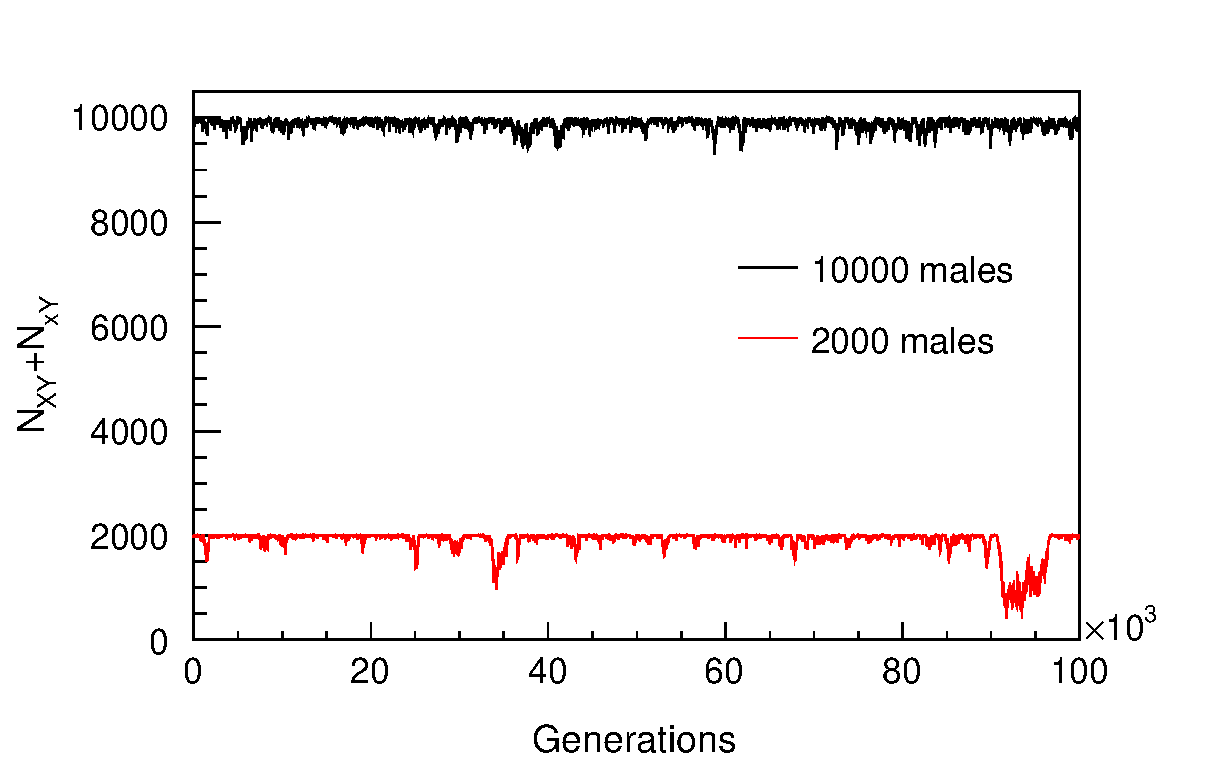
\includegraphics[width=8.6cm]{cpp/X-linked/c1.eps}
      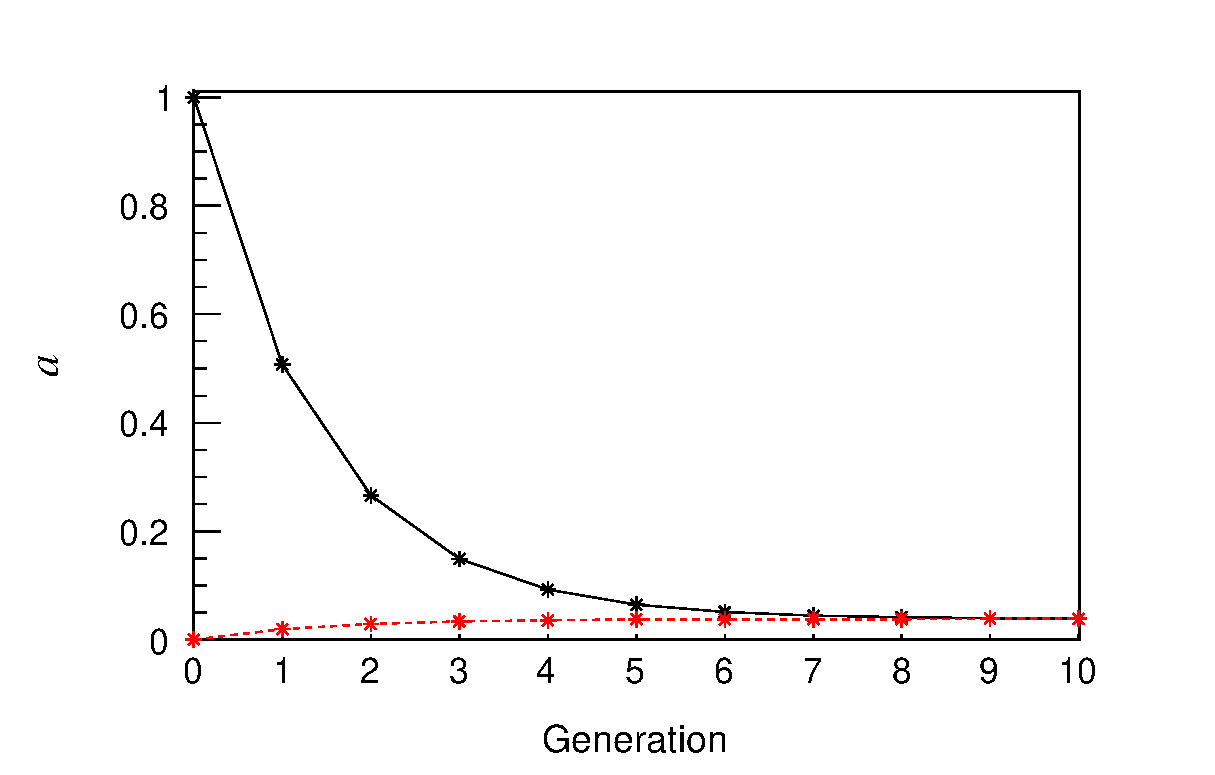
\includegraphics[width=8.6cm]{Fig1.eps}
      \caption{
Two examples of the evolving of $a$ for X-linked locus, with initial values 1 and 0, respectively, where $a$ is the frequency of genotype Gg. Both examples converge to equilibrium $\frac{1+4\mu-\sqrt{1+8\mu}}{2\mu}\approx 4\mu$, where $\mu$ is the mutation rate from the allele G to the allele g per generation. We choose $\mu=10^{-2}$ for demonstration purposes.
}\label{X_linked}
\end{figure}

Frequency $a$ converges with respect to generation, as demonstrated in Fig. \ref{X_linked}, and when the equilibrium is reached, there will be an equation
\begin{equation}
a=\frac{4 \mu + a - 2 \mu a }{2 + 2 \mu - \mu a  },
\end{equation}
which reflects mutation-selection balance.
Under the constraint of $0\le a\le 1$, the equation has only one solution,
\begin{equation}\label{4mu}
	a=\frac{1+4\mu-\sqrt{1+8\mu}}{2\mu},
\end{equation}
which is approximately $a\approx 4\mu$ when $\mu\ll 1$.
If male individuals of genotype g are alive but infertile, their corresponding frequency would be $\frac{a}{2}+\left[\frac{a}{2}+(1-a)\right]\mu$, or approximately $2\mu + \mu$,
where $2\mu$ is inherited and $\mu$ is {\it de novo} mutation. This is the same result that has been obtained by Haldane \citep{Haldane2004a}. The frequency of the g allele can also be calculated, and it is approximately $\frac{4}{3} \mu$, in contrast to the result $3\mu$ derived from Hardy-Weinberg equilibrium \citep{johnston2019population}. The discrepancy reflects that the Hardy-Weinberg population does not apply when the mutation is considered. 

\section{Autosomal locus}
Consider an autosomal locus with alleles G and g. Let $\mu$ represent the mutation rate from G to g per generation, with no difference between males and females and no back mutation. Suppose the population is large and mating is at random.  The genotypes are GG, Gg, and gg. Let their relative fitnesses be 1, 1, and 0, respectively. Let us denote the frequency of genotype Gg by $a$, with no difference between males and females. The reproduction process is shown in Table \ref{autosome}, where no mutation is considered.
\begin{table}[htp]
        \caption{Reproduction with no mutation considered. The relative fitnesses of genotypes GG, Gg, and gg are 1, 1, and 0, respectively. The frequencies of genotypes GG and Gg for parental generation are $1-a$ and $a$, respectively. 
\label{autosome}
        }
        \begin{center}
                \begin{tabular}{ c!{\vrule width 1pt}c|c|c }
                        \hline
                        \vspace{-2mm}
                             &     &     &     \\
       			%\diaghead{2,2}{female}{male} & GG    & Gg    & gg    \\
       			& GG    & Gg    & gg    \\
                        & $1\!-\!a$ & $a$     &       \\
                        \vspace{-3mm} &       &     \\
			\noalign{\hrule height 1pt}
                        \vspace{-2mm}
                        &     &     &       \\
                        GG      & \{ 4GG \} & \{ 2GG, 2Gg \}   &-      \\
                        $1\!-\!a$     & $(1\!-\!a)^2$  & $(1\!-\!a)a$          &       \\
                        \vspace{-3mm}      &     &     &     \\
                        \hline
                        \vspace{-2mm}
                        &     &     &          \\
                        Gg      & \{ 2GG, 2Gg \}   & \{ GG, 2Gg, gg \}  &-      \\
                        $a$       & $a(1\!-\!a)$      & $a^2$      &       \\
                        \vspace{-3mm} &          &     &     \\
                        \hline
                        \vspace{-2mm}
                        &     &     &          \\
                        \ \ \ \ \ gg\ \ \ \ \       &\ \ \ \ \ \ \ \ \ \ \ \ \ - \ \ \ \ \ \ \ \ \ \ \ \ \    & \ \ \ \ \ \ \ \ \ \ \ \ \ - \ \ \ \ \ \ \ \ \ \ \ \ \     & \ \   - \ \ \         \\
                        \hline
                \end{tabular}
        \end{center}
\end{table}

To take into account mutation, we plug Eqs. (\ref{GG}) and (\ref{Gg}) into Table (\ref{autosome}). Thus, we get
\begin{equation}
 \begin{array}{lll}
\vspace{2mm} N_{\rm GG}\propto&\left[4(1-a)^2+4a(1-a)+a^2\right](1-\mu)^2,\\
\vspace{2mm} N_{\rm Gg}\propto&\left[4(1-a)^2+4a(1-a)+a^2\right]2\mu(1-\mu)\\
\vspace{2mm} &+\left[4a(1-a)+2a^2\right](1-\mu),
  \end{array}
  \vspace{3mm}
\end{equation}
where $N_{\rm GG}$ and $N_{\rm Gg}$ are the numbers of offspring individuals with genotypes GG and Gg, respectively. Let us introduce $a_n$ for parents and $a_{n+1}$ for offspring. Then we have
\begin{equation}
a_{n+1}=\frac{8 \mu + 4a_n - 8 \mu a_n -  2a_n^2 + 2\mu a_n^2}{4 + 4 \mu - 4\mu a_n - a_n^2 + \mu a_n^2 }.
\end{equation}

\begin{figure}
      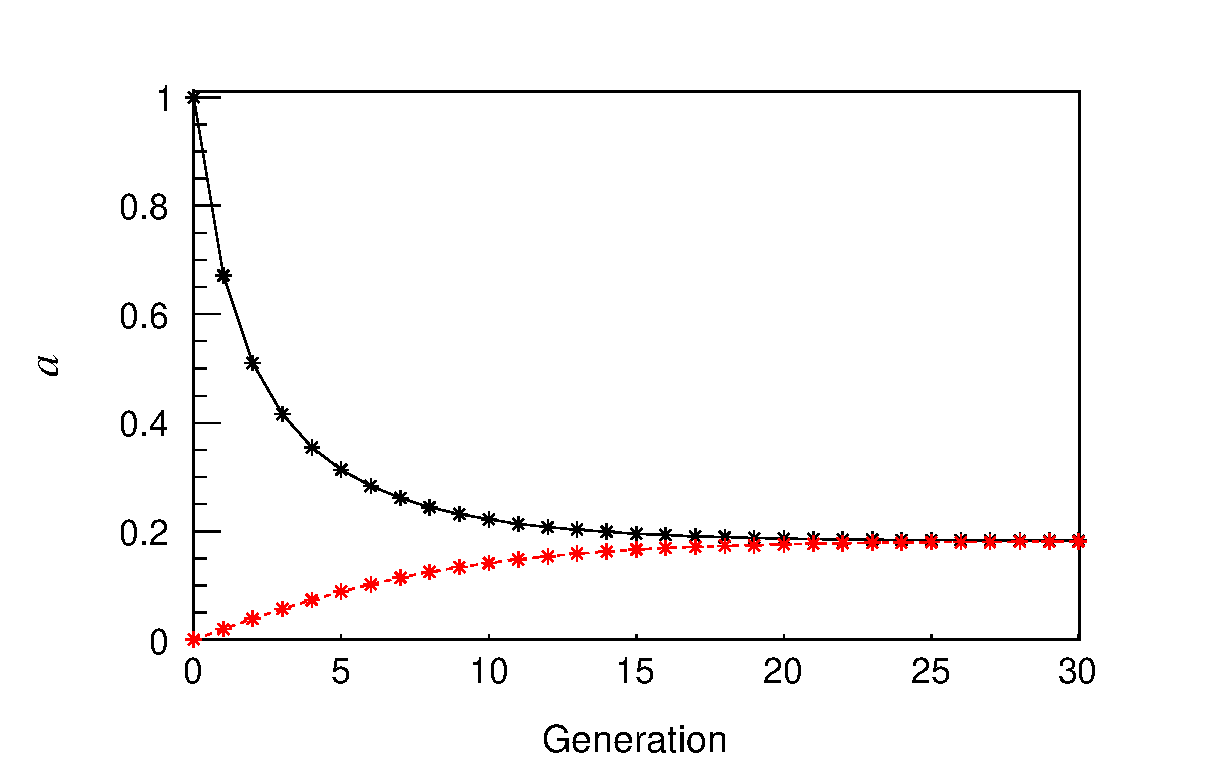
\includegraphics[width=8.6cm]{Fig2.eps}
      \caption{
Two examples of the evolving of $a$ for autosomal locus, with initial values 1 and 0, respectively, where $a$ is the frequency of genotype Gg. Both examples converge to equilibrium $2\frac{\sqrt{\mu}-\mu}{1-\mu}\approx 2\sqrt{\mu}$ where $\mu=10^{-2}$ for demonstration purposes.
}\label{auto}
\end{figure}


Frequency $a$ will converge, as demonstrated in Fig. \ref{auto}, and equilibrium will be reached, satisfying equation
\begin{equation}
        a=\frac{8 \mu + 4a - 8 \mu a -  2a^2 + 2\mu a^2}{4 + 4 \mu - 4\mu a - a^2 + \mu a^2 }.
\end{equation}
Under the constraint of $0\le a\le 1$, the equation has only one solution,
\begin{equation}\label{2sqrtmu}
        a =2\frac{\sqrt{\mu}-\mu}{1-\mu}.
\end{equation}
We may further obtain the frequency of allele g as $\frac{\sqrt{\mu}-\mu}{1-\mu}$. When  $\mu\ll 1$, it is approximate $\sqrt{\mu}$, which is the same as the result obtained based on the Hardy-Weinberg law \citep{johnston2019population}. 

\section{X-degenerate gene}
The role of the X chromosome is essential in Y-chromosome degeneration. Engelst\"{a}dter \citep{engelstadter2008muller}, by simulation, showed that mutations arising on the X chromosome cause strong selection against mutations on the Y chromosome, reducing the speed of Y-chromosome degeneration. 
For this reason, we study the X and Y chromosomes together.

Let us extend Haldane's approach to a locus that is non-sex-specific and located within a non-recombining region on both X and Y chromosomes. Suppose that the locus has alleles G and g. Let $\mu$ represent the mutation rate from G to g per generation, with no difference between males and females and no back mutation. Suppose the population is large and mating is at random. 
Let us introduce the following symbols:
\begin{itemize}
\itemsep=0pt \parskip=0pt
\item X --	  X chromosome with G;
\item x -- 	  X chromosome with g;
\item Y --	  Y chromosome with G;
\item y -- 	  Y chromosome with g;
\vspace{1mm}
{
\item $ a=\frac{N_{\rm Xx}}{N_{\rm XX}+N_{\rm Xx}}$ }; 
\vspace{1mm}
{
\item $ b=\frac{N_{\rm Xy}}{N_{\rm XY}+N_{\rm Xy}+N_{\rm xY}}$}; 
\vspace{1mm}
{
\item $ c=\frac{N_{\rm xY}}{N_{\rm XY}+N_{\rm Xy}+N_{\rm xY}}$}; 
\end{itemize}
where $N_{\rm XX}$ refers to the number of individuals of genotype XX, and so on. 
The fitness is 1 for genotypes XX, Xx, XY, Xy, xY and 0 for xx and xy.
The reproduction process is shown in Table \ref{XY}, where no mutation is considered. 

\begin{table*}[]
	\caption{
Reproduction with no mutation considered. For males, the relative fitnesses of XY, Xy, xY, xy are 1, 1, 1, 0, respectively. The relative fitnesses of genotypes XX, Xx, xx for females are 1, 1, 0, respectively. The frequencies of genotypes XY, Xy, xY are $1\!-b-c$, $b$, $c$, respectively. The frequencies of genotypes XX and Xx are $1\!-a$ and $a$, respectively.
\label{XY}
	}
	\begin{center}
		\begin{tabular}{ c!{\vrule width 1pt}c|c|c|c }
			\hline
			\vspace{-2mm}
			&     &     &     &     \\
			& XY    & Xy    & xY    & xy    \\
			& $1\!-\!b\!-\!c$ & $b$     & $c$     &       \\
			\vspace{-3mm} &     &     &     &     \\
			\noalign{\hrule height 1pt}
			\vspace{-2mm}
			&     &     &     &     \\
			XX      & \{ 2XX, 2XY\} & \{ 2XX, 2Xy \}        & \{ 2Xx, 2XY \}        &-      \\
			$1\!-\!a$     & $(1\!-\!a)(1\!-\!b\!-\!c)$  & $(1\!-\!a)b$                & $(1\!-\!a)c$                &       \\
			\vspace{-3mm} &     &     &     &     \\
			\hline
			\vspace{-2mm}
			&     &     &     &     \\
			Xx      & \{ XX, Xx, XY, xY\}   & \{ XX, Xx, Xy, xy \}  & \{ Xx, xx, XY, xY \}  &-      \\
			$a$       & $a(1\!-\!b\!-\!c)$      & $ab$            & $ac$            &       \\
			\vspace{-3mm} &     &     &     &     \\
			\hline
			\vspace{-2mm}
			&     &     &     &     \\
			xx      & -     & -     & -     &\ \ \  -\  \ \ \ \        \\
			\hline
		\end{tabular}
	\end{center}
\end{table*}

We plug the following into Table \ref{XY} to account for mutation. 
\begin{equation} \label{1}
  \begin{array}{lllll}
  {\rm XX}&\to 
  \begin{cases}
    {\rm XX}, &(1-\mu)^2,\\ {\rm Xx}, &2\mu(1-\mu),\\{\rm xx}, &\mu^2 ; 
  \end{cases}
  \end{array} 
\end{equation}
\vspace{-0.5cm}
\begin{equation} \label{2}
  \begin{array}{lllll}
  {\rm XY}&\to 
  \begin{cases}
   {\rm XY}, &(1-\mu)^2,\\ {\rm Xy}, &\mu(1-\mu),\\ {\rm xY}, &\mu(1-\mu),\\ {\rm xy}, &\mu^2 ;
  \end{cases}
  \end{array} 
\end{equation}
\vspace{-0.0cm}
\begin{equation} \label{3}
  \begin{array}{lllll}
   {\rm Xx}&\to 
  \begin{cases}
  {\rm Xx}, &(1-\mu),\\  {\rm xx}, &\mu; \\
  \end{cases} 
  \end{array} 
\end{equation}
\vspace{-0.0cm}
\begin{equation} \label{4}
  \begin{array}{lllll}
	{\rm Xy}&\to 
	\begin{cases}
    		{\rm Xy}, &(1-\mu),\\ {\rm xy}, &\mu;
	\end{cases}
  \end{array} 
\end{equation}
\vspace{-0.0cm}
\begin{equation} \label{5}
\begin{array}{lllll}
 {\rm xY}&\to 
  \begin{cases}
  {\rm xY}, &(1-\mu),\\{\rm xy}, &\mu.
  \end{cases}
  \end{array} 
\end{equation}
 Let us introduce $a_n,b_n,c_n$ for parents and $a_{n+1}$, $b_{n+1}$, $c_{n+1}$ for offspring.
Then we have
{\begin{equation}\label{np1} 
 \begin{array}{lll}
\vspace{3mm}
a_{n+1}=\frac{  4 \mu + a_n - 2 \mu a_n + 2 c_n - 4 \mu c_n - 2 a_n c_n + 2 \mu a_n c_n}{2 + 2 \mu - \mu a_n - 2 \mu c_n - a_n c_n + \mu a_n c_n },\\
\vspace{3mm}
b_{n+1}= \frac{ 2 \mu - \mu a_n +2 b_n - 2 \mu b_n - a_n b_n + \mu a_n b_n }{2 + 2 \mu - \mu a_n - 2 \mu b_n - a_n b_n + \mu a_n b_n },\\
c_{n+1}=\frac{2 \mu+ a_n  - \mu a_n - 2 \mu b_n - a_n b_n + \mu a_n b_n}{2 + 2 \mu - \mu a_n - 2 \mu b_n - a_n b_n + \mu a_n b_n }.
  \end{array} 
\end{equation}
}

Variables $(a,b,c)$ converge with respect to generation. Equilibria exist, satisfying
{\begin{equation} 
\left\{
  \begin{array}{lll}
\vspace{3mm}
a=\frac{  4 \mu + a - 2 \mu a + 2 c - 4 \mu c - 2 a c + 2 \mu a c}{2 + 2 \mu - \mu a - 2 \mu c - a c + \mu a c },\\
\vspace{3mm}
b= \frac{ 2 \mu - \mu a +2 b - 2 \mu b - a b + \mu a b }{2 + 2 \mu - \mu a - 2 \mu b - a b + \mu a b },\\
c=\frac{2 \mu+ a  - \mu a - 2 \mu b - a b + \mu a b}{2 + 2 \mu - \mu a - 2 \mu b - a b + \mu a b }.
  \end{array} 
\right.
\end{equation}
}
Under the constraints $0\leq a,b,c\leq 1$, the equation has two solutions, giving rise to two equilibria. The first equilibrium is
\begin{equation}\label{firstsolution} 
	\begin{array}{lll}
	(a,b,c)&=&\left(2\frac{\sqrt{\mu}-\mu}{1-\mu},\ \frac{\sqrt{\mu}-\mu}{1-\mu},\ \frac{\sqrt{\mu}-\mu}{1-\mu}\right)\\
		 &\approx & ( 2\sqrt{\mu},\ \sqrt{\mu},\ \sqrt{\mu}).
	\end{array}
\end{equation}
The second equilibrium is
\begin{equation}\label{secondsolution} 
	\begin{array}{lll}
	(a,b,c)&=&\left(\frac{1+4\mu-\sqrt{1+8\mu}}{2\mu},\ 1,\ 0\right)\\
		 &\approx &( 4\mu,\ 1,\ 0).
	\end{array}
\end{equation}
The first equilibrium is the same as the equilibrium (\ref{2sqrtmu}) in the scenario of autosomal locus. The second equilibrium is the same as the equilibrium (\ref{4mu}) in the scenario of X-linked locus. 

When the G allele is dosage sensitive, the genotype Xy will be subject to additional selective pressure, resulting in an even lower frequency $b$. But equilibria still exist. It is argued \citep{charlesworth1978model} that the presence of the genotype Xy would trigger dosage compensation. However, in the first equilibrium, the frequency of genotype Xy is too low to trigger such a mechanism, given that the dominant genotype is XY and the dosage compensation would be harmful to XY. However, this mechanism should apply to the second equilibrium where the only genotype is Xy, and dosage compensation is free to develop for males.  

For given variables $(a_n,b_n,c_n)$, only when $b_n=1$ the coming generations converge to the second equilibrium; otherwise, they always converge to the first equilibrium, regardless of $a_n$ and $c_n$. In other words, if the allele G is present on Y at the beginning, it is always present. 

The existence of the equilibria, especially the first equilibrium, means that Y-chromosome degeneration does not happen as long as the population is large. However, equilibrium can easily be disturbed when the population size is small, possibly resulting in Y-chromosome degeneration. To study this possibility, let us take the first equilibrium and randomly choose a small population from it.

\section{Small population size}
Let us extend the relations in Table \ref{XY} to a finite population. A simulation can do this, as shown in the appendix. For demonstration purposes, we choose mutation rate $\mu=10^{-4}$ and a binomial sampling method. Fig. \ref{figure9} shows that fluctuations may dominate over equilibrium when the population is not large. Fig. \ref{figure7} shows that Muller's ratchet may click when the population is small, as a reflection of the population bottleneck effect \citep{Weaver2021}. Such events may have occurred to species of small-sized populations, e.g., frogs from Caribbean islands \citep{Ma2021}. Meanwhile, a large population should be able to keep every remaining active gene on the Y chromosome, e.g., humans \citep{tomaszkiewicz2016time}.

\begin{figure}
      \includegraphics[width=8.6cm]{Fig3.eps}
      \caption{
Two examples of the Y chromosome evolving, with 10,000 and 2000 males participating in reproduction, respectively. On the vertical axis is the total number of individuals of genotypes XY and xY. Fluctuations are apparent, but each example's equilibrium position is also apparent. The sampling method is the binomial sampling that is used in the Wright-Fisher model \citep{Muirhead2016}. The mutation rate is $\mu=10^{-4}$ for demonstration purposes. 
Competition exists between mutation-selection balance and sampling randomness. When the mutation rate is lower, e.g., $\mu=10^{-5}$ or $\mu=10^{-6}$, the competition will result in wider windows switching between equilibrium and fluctuations seen in the Wright-Fisher model.
}\label{figure9}
\end{figure}

\begin{figure}
      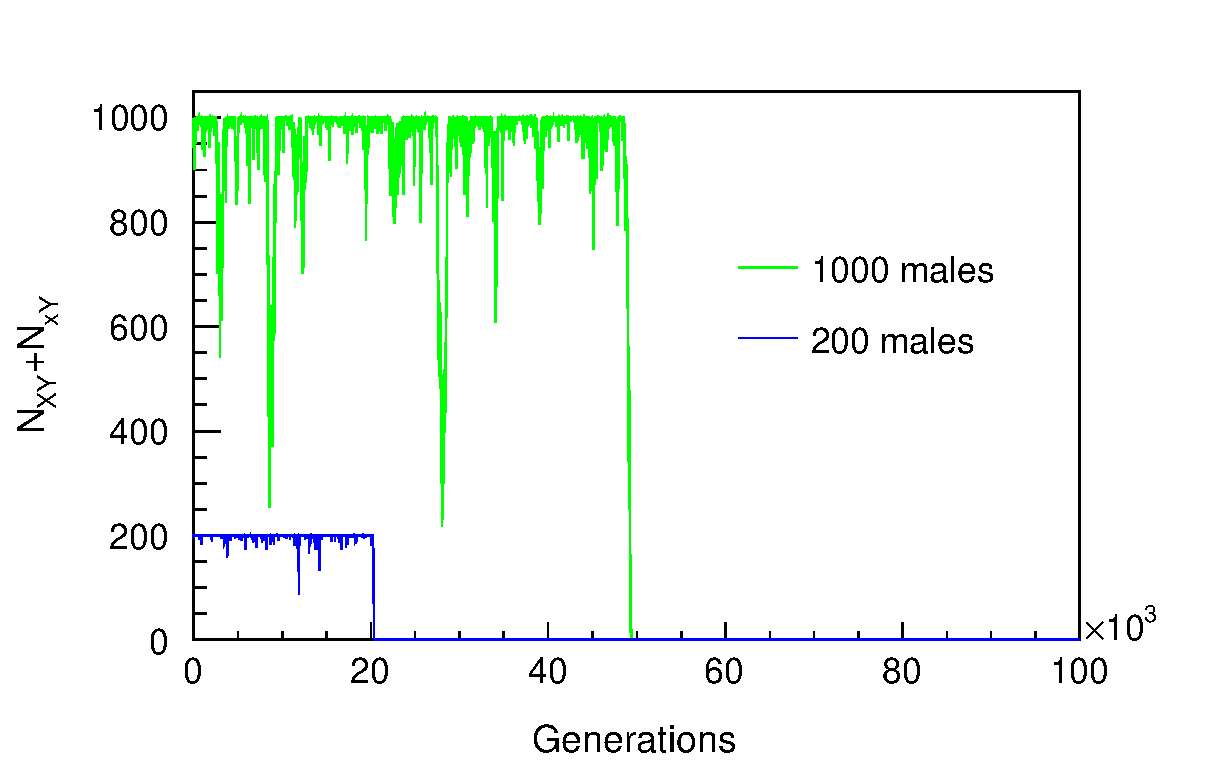
\includegraphics[width=8.6cm]{Fig4.eps}
      \caption{
Two examples of the Y chromosome evolving, with 1000 and 200 males participating in reproduction, respectively. The mutation rate is $\mu=10^{-4}$ for demonstration purposes. Fluctuations are significant, and Muller's ratchet clicks at generations 20,360 and 49,369, respectively.
}\label{figure7}
\end{figure}


\section{Founder effect}
Founder effect \citep{templeton1980theory,provine2004ernst,joly2011existence} should play a more critical role. Consider a one-male scenario where: (1) the first generation has one male; (2) the second generation has two or more males, and so on until the population is large. In this scenario, the probability of finding genotype XY/xY in any generation is nearly a constant, $1-\frac{\sqrt{\mu}-\mu}{1-\mu}$, which is $\approx 0.99$ when $\mu=10^{-4}$. For a scenario where the population starts with two males or more, the probability will be increased to 0.9999 or higher, which, by comparison, gives rise to negligible contributions to Y-chromosome degeneration. 

Let us apply the one-male scenario to a chain of peripatric speciation \citep{Colvin2018} events: species $\alpha$ $\to$ species $\beta$ $\to$ species $\gamma$ $\to \ \cdots$. Species $\beta$ has the probability of 0.99 of having XY/xY; species $\gamma$ has the probability of $0.99^2$ of having XY/xY, and so on. After 70 such founder events, the probability is down to $0.99^{70}\approx 0.5$. In other words, the Y chromosome has a 50\% probability of having only the g allele after 70 such speciation events. When $\mu=10^{-6}$, to reach the same probability would need 700 such speciation events. When the Y chromosome has only g allele, the allele can still pass on for many generations, but it will lose base pairs little by little, shortening the Y chromosome. 

A species may have gone through many speciation events that are affected by the founder effect. The tendency is that the more advanced a species is, the more such events may have happened, and the more X-degenerate genes may have become lost from the Y chromosome.

\section{Conclusions}
For a large population, equilibrium can be established for non-sex-specific alleles located within non-recombining regions on both X and Y chromosomes. In other words, when the population is large, the Y chromosome can retain its active genes without experiencing degeneration. 
%However, Muller's ratchet may click for small populations due to the population bottleneck effect. %For average population size, the effect should be negligible.
The existence of the equilibrium for a large population means that there is always a tiny fraction of the male population carrying some inactive allele of a gene instead of the active allele. If such a male gives rise to a new species, the species will only have the inactive allele on the Y chromosome, which will become shorter when the inactive allele is lost. 
%The inactive allele on the Y chromosome will eventually lose its base pairs, resulting in a shortened Y chromosome. 
%This type of Y degeneration occurs throughout speciation instead of over generations. 
Primitive species, such as frogs, may have gone through few founder events and therefore have long Y chromosomes; advanced species, like humans, should have gone through many founder events and therefore have short Y chromosomes.
% that do not become shorter.  % retain the remaining active genes on the Y chromosome.

\section*{Statements and Declarations}
\vspace{0.2cm}
\noindent {\large\bf Data accessibility}

\vspace{0.2cm}
\noindent {Simulation code repository: https://github.com/zyjlntu/Y-degeneration}

\noindent {This article does not contain any additional data.}

\vspace{0.2cm}
\noindent {\large\bf Competing interests}

\vspace{0.2cm}
\noindent {We declare we have no competing interests.}


\vspace{0.2cm}
\noindent {\large\bf Funding}

\vspace{0.2cm}
\noindent {We received no funding for this study.}

\begin{appendices}
%\appendix*
\section{Simulation}
Simulation is necessary when the relations in Table \ref{XY} are applied to a finite population.
Fig. \ref{flowchart} is the flowchart of the main program.
Fig. \ref{males} is the subroutine flowchart of reproducing female offspring. Reproducing males is done similarly.

\begin{figure}
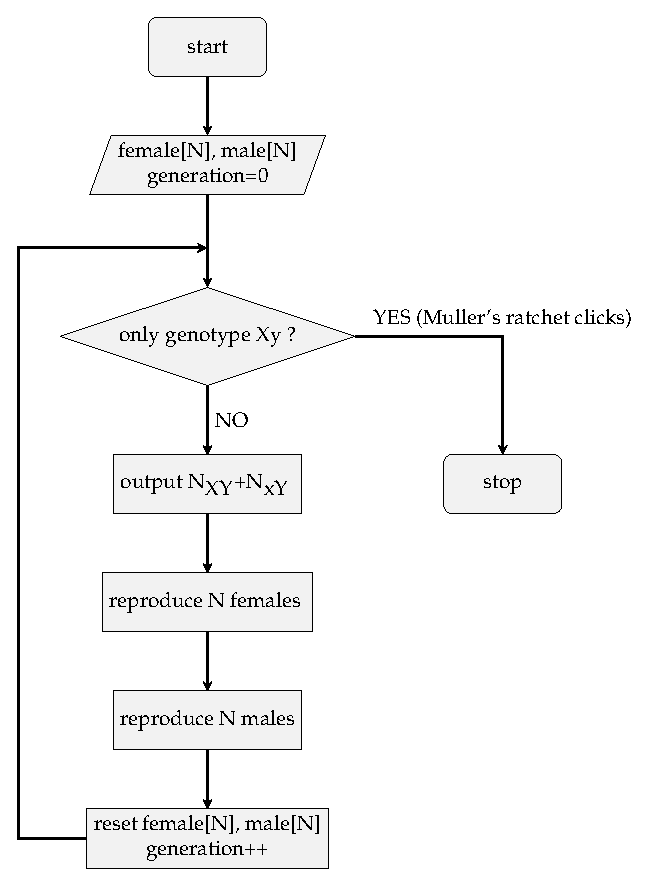
\includegraphics[width=6cm]{FigA1.eps} 
\caption{ 
The flowchart of the main program (C++) for simulation. The first generation of N males and N females are randomly chosen from the first equilibrium (\ref{firstsolution}). If all N males happen to be genotype Xy, the program stops. Otherwise, the next generation is reproduced, and so on. When the program stops, it means that Muller's ratchet clicks.
By printing N$_{\rm XY}$+N$_{\rm xY}$, Fig. \ref{figure9}, and Fig. \ref{figure7} are produced. 
}\label{flowchart}
\end{figure}

\begin{figure}
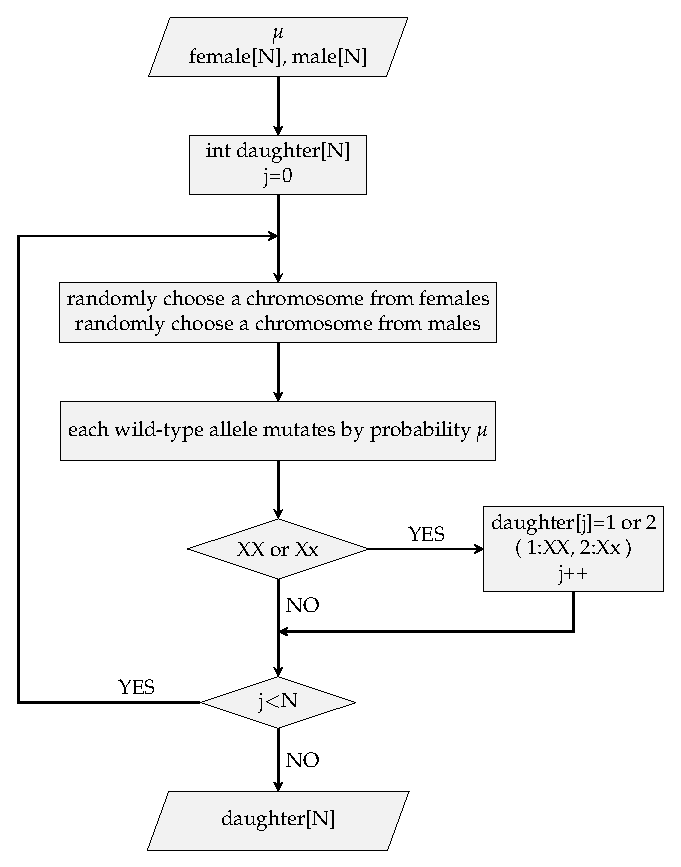
\includegraphics[width=7cm]{FigA2.eps} 
\caption{ 
The flowchart of the program reproducing females. The input is N females and N males; the output is N females. 
Males can be reproduced similarly. The sampling method is the binomial sampling that is used in the Wright-Fisher model, in which fluctuations are more significant due to the lack of mutation and selection.  
}\label{males}
\end{figure}

\end{appendices}

\bibliography{library}

\end{document}


